% --------------------------------------------------------------------------------------------------
% Section: Model Architecture
% --------------------------------------------------------------------------------------------------
\section{Model Architecture}

% Introductory statement highlighting the use of CNNs in medical imaging for lung cancer
Lung cancer detection using \textbf{Convolutional Neural Networks (CNNs)} has become a promising 
approach in medical imaging due to CNNs’ ability to automatically learn and extract relevant 
features from complex CT scan images.

% --------------------------------------------------------------------------------------------------
% Subsection: Overview of CNN structure
% --------------------------------------------------------------------------------------------------
\subsection{Overview of CNN structure (layers, activations)}

\begin{itemize}
    % Core building block of CNNs: Convolutional layers
    \item \textbf{Convolutional Layers}: These layers form the core of the CNN architecture. Each 
    convolutional layer applies multiple filters (kernels) to the input or previous layer’s feature 
    maps to detect local patterns such as edges, textures, and shapes relevant to lung cancer.

        \begin{itemize}
            % Filters used for scanning the image to detect features
            \item \textbf{Filter size}: Typically 3×3 filters are used because they strike a balance 
            between capturing fine-grained details and computational efficiency. \cite{sr2025}

            % Number of filters per layer, increasing to capture more complex features
            \item \textbf{Number of filters}: The number of filters usually increases progressively 
            through the network (e.g., 32, 64, 128, 256), allowing the model to learn from simple to 
            complex features hierarchically.

            % Deeper architectures allow detection of subtle patterns
            \item \textbf{Stacked convolutions}: Multiple convolutional layers are stacked to deepen 
            the network, enabling the detection of subtle malignancies and complex lung tissue 
            patterns.
        \end{itemize}

    % Explains the role of convolutional layers in detecting lung cancer
    The convolutional layers are vital for extracting meaningful features from the CT scans, which 
    are critical for distinguishing between normal, benign, and malignant tissues.

    % Convolutional layer visualization
    \vspace{1em}
    \begin{center} 
        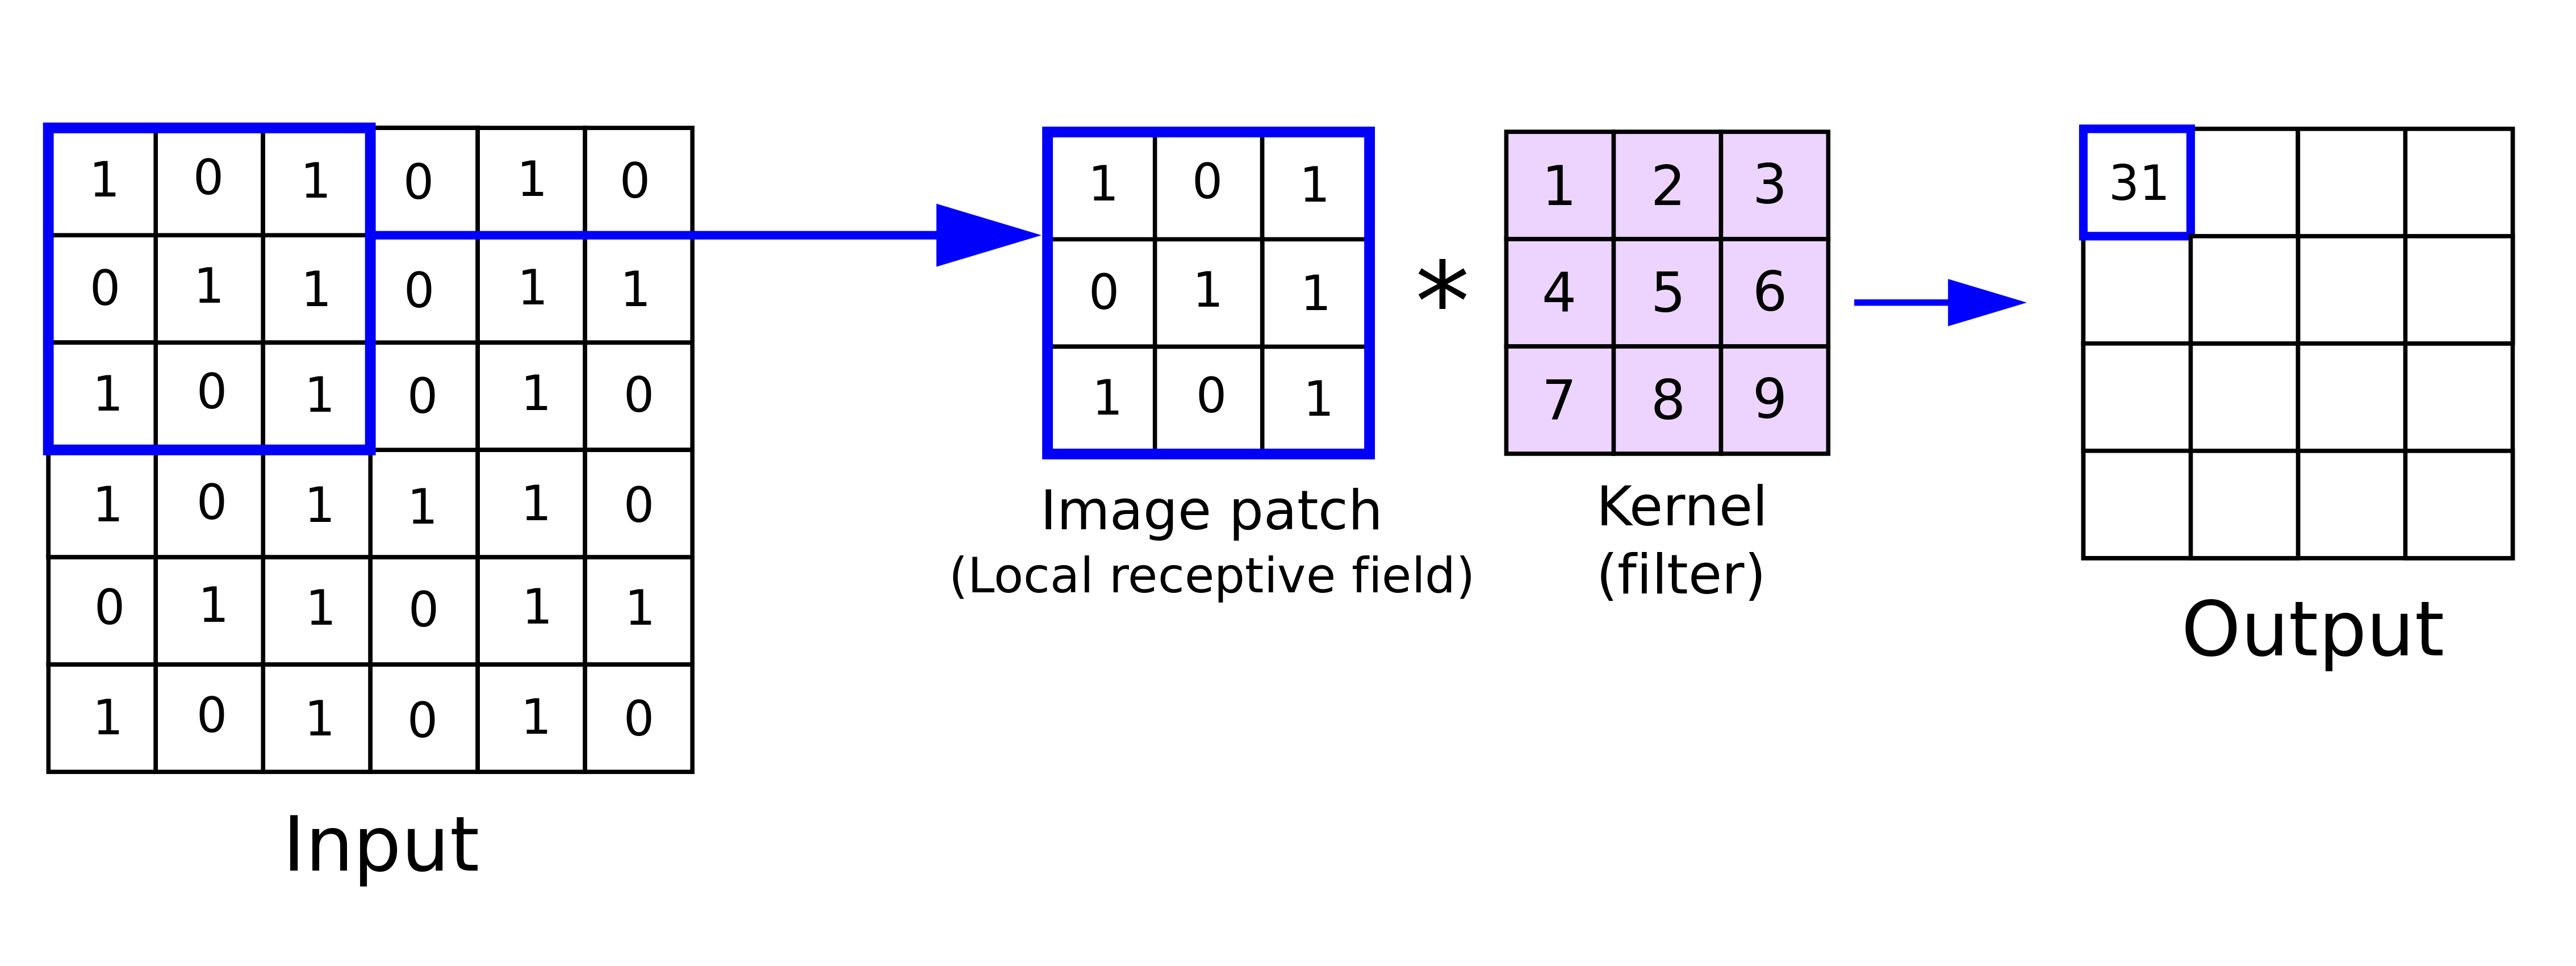
\includegraphics[width = 0.8\textwidth]
        {../assets/03-model-architecture/convolutional-layer.png}

        \small\textit{Convolutional layer representation. \cite{ar2019}}
    \end{center}
    \vspace{1em}

    % Batch Normalization layer helps with model stability and training speed
    \item \textbf{Batch Normalization}: After each convolutional operation, batch normalization 
    layers are inserted to normalize the activations. This technique stabilizes and accelerates 
    training by reducing internal covariate shift, which helps the model converge faster and 
    generalize better on unseen data.\cite{sr2025}

    % Non-linear activations are critical for learning complex patterns
    \item \textbf{Activation Functions}: The Rectified Linear Unit (ReLU) activation function is 
    applied after batch normalization in each convolutional block. ReLU introduces non-linearity by 
    outputting zero for negative inputs and the input itself for positive values.

        \begin{itemize}
            % ReLU helps prevent vanishing gradients
            \item \textbf{Impact}: ReLU prevents the vanishing gradient problem, allowing deeper 
            networks to learn effectively.

            % ReLU contributes to faster learning
            \item \textbf{Training efficiency}: It speeds up convergence during training.
            
            % ReLU enhances feature extraction
            \item \textbf{Feature learning}: Enables the network to learn complex, non-linear 
            features essential for accurate lung cancer classification. \cite{sr2025}
        \end{itemize}

    % Pooling reduces size and increases robustness
    \item \textbf{Pooling Layers}: Max pooling layers with a typical pool size of 2×2 are inserted 
    after convolutional blocks to downsample the feature maps.

        \begin{itemize}
            % Pooling helps lower memory and computation needs
            \item \textbf{Purpose}: Reduce spatial dimensions, lowering computational load.
            
            % Adds robustness to small input variations
            \item \textbf{Robustness}: Provides translation invariance, making the model less 
            sensitive to small shifts or distortions in lung images.

            % Retains only the most important features in regions
            \item \textbf{Information retention}: Max pooling preserves the most prominent features 
            in each region, which is crucial for detecting cancerous nodules.
        \end{itemize}

    % Visualization of max pooling process
    \vspace{1em}
    \begin{center} 
        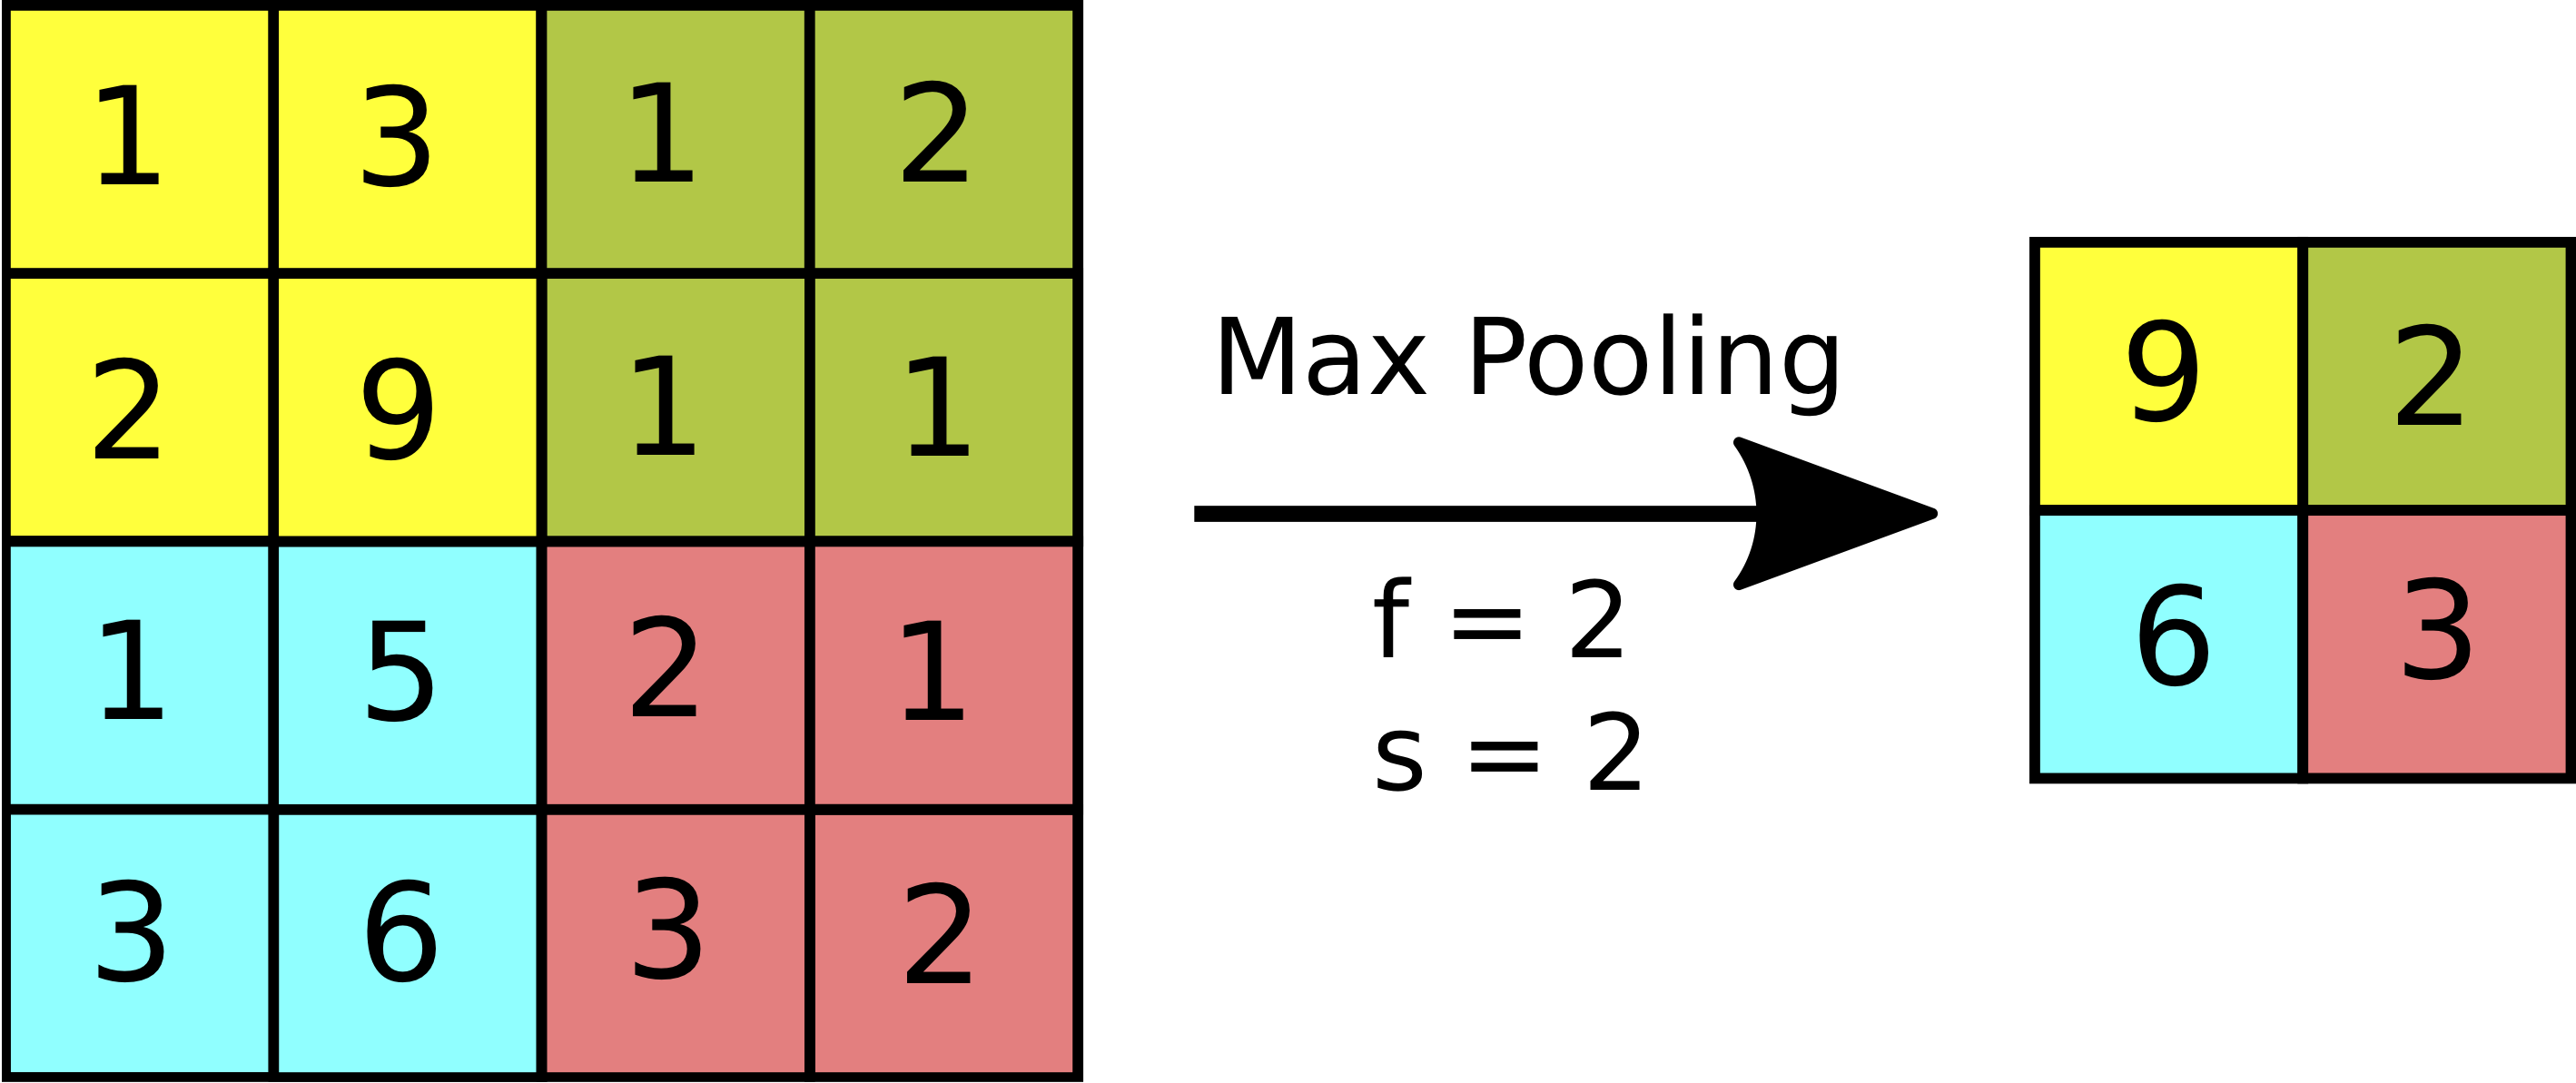
\includegraphics[width = 0.5\textwidth]{../assets/03-model-architecture/max-pooling.png}

        \small\textit{Max pooling representation. \cite{ar2019}}
    \end{center}
    \vspace{1em}

    % Dropout improves generalization by reducing overfitting
    \item \textbf{Dropout Layers}: Dropout layers randomly deactivate a fraction of neurons during 
    training (commonly 0.5 dropout rate). This prevents the network from overfitting by forcing it 
    to learn redundant and more robust feature representations. These layers are particularly 
    important in medical imaging, where datasets may be limited and overfitting is a risk.

    % Flatten prepares the features for classification
    \item \textbf{Flatten Layer}: After the convolutional and pooling layers, the multi-dimensional 
    feature maps are flattened into a one-dimensional vector. This transformation prepares the data 
    for the fully connected layers that perform the final classification.

    % Dense layers are used to integrate features and predict outcomes
    \item \textbf{Dense Layer}: One or more fully connected layers follow the flattening step. 
    These layers integrate all extracted features to make a final decision on the presence and type 
    of lung cancer. Dense layers typically contain hundreds of neurons to capture complex feature 
    interactions.
\end{itemize}

% Diagram showing full CNN architecture for reference
\vspace{1em}
\begin{center} 
    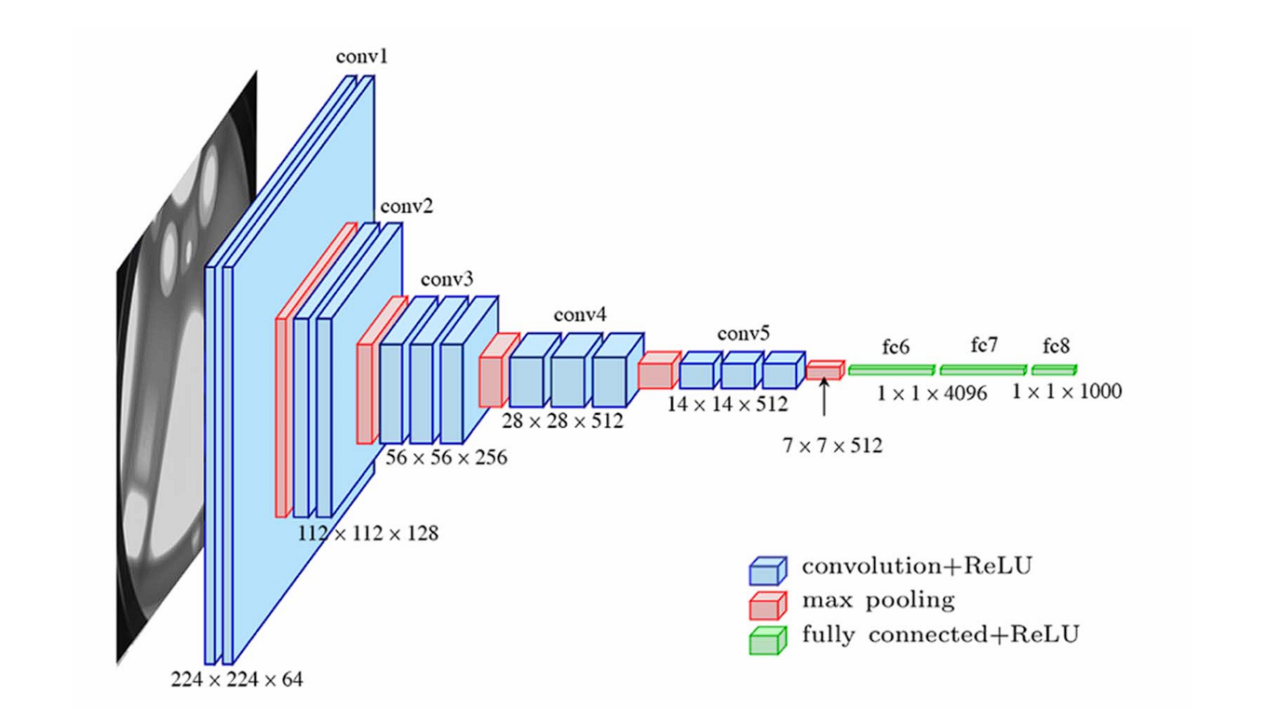
\includegraphics[width = \textwidth]{../assets/03-model-architecture/cnn-diagram.png}

    \small\textit{Diagram of Very Deep Convolutional Networks. \cite{vcg2021}}
\end{center}
\vspace{1em}

% --------------------------------------------------------------------------------------------------
% Subsection: Input/output format
% --------------------------------------------------------------------------------------------------
\subsection{Input/output format}

\begin{itemize}
    % Input preprocessing and format for consistency and quality
    \item \textbf{Input Layer and Preprocessing}: The CNN model begins with an input layer designed 
    to accept lung CT scan images resized to a standardized dimension, often 256×256 pixels. This 
    resizing ensures consistent input size for the network and preserves critical spatial 
    information necessary for detecting lung nodules or tumors. Preprocessing steps prior to input 
    include noise reduction (techniques such as thresholding and segmentation are applied to remove 
    irrelevant regions like bones, air, and background noise, isolating lung tissues for focused 
    analysisand) and contrast enhancement to improve image quality while avoiding loss of important 
    features.\cite{aplb2024}

    % Output prediction types: binary or multiclass classification
    \item \textbf{Output Layer and Prediction}: 
        \begin{itemize}
            % Binary: cancerous vs non-cancerous
            \item \textbf{Binary classification}:
                \begin{itemize}
                    \item \textbf{Structure}: A single neuron with a sigmoid activation (e.g., 
                    cancerous vs. non-cancerous).
                    
                    \item \textbf{Output}: A scalar value between 0 and 1 representing the 
                    probability that the input image contains cancerous tissue. A threshold 
                    (commonly 0.5) is applied to convert the probability into a class label 
                    (e.g., benign if probability less than 0.5, malignant otherwise).
                \end{itemize}

            % Multiclass: normal, benign, malignant, etc.
            \item \textbf{Multiclass classification}: 
                \begin{itemize}
                    \item \textbf{Structure}: Multiple neurons equal to the number of classes (e.g., 
                    normal, benign, malignant) with a softmax activation function.
                    
                    \item \textbf{Output}: A probability distribution over all classes, where the 
                    sum of probabilities equals 1. The class with the highest probability is 
                    selected as the predicted label. For example, if the output is [0.1, 0.7, 0.2], 
                    the model predicts “benign” with 70\% confidence.
                \end{itemize}
            
            % Output confidence calibration for clinical reliability
            \item \textbf{Confidence Scores}: The output probabilities provide a measure of 
            confidence in the prediction. This is essential for clinical applications where 
            uncertain cases may require further examination or additional testing. Well-calibrated 
            models produce probabilities that accurately reflect true likelihoods. Calibration 
            techniques such as Platt scaling or isotonic regression may be applied post-training to 
            improve reliability.
        \end{itemize}
\end{itemize}
